\section{Den bagvedlæggende kemi}

Her har du brug for harmoniske svingninger \ref{teori: Harmoniske svingninger}

Stort set alle kemiske forbindelser, der indeholder kovalente bindinger absorberer nogle specielle frekvenser af elektromagnetisk stråling i den infrarøde del af det elektromagnetiske spektrum. Det infrarøde lys har en længere bølgelængde en det lys menneskets øjne kan opfange $400nm - 800nm$ men kortere end det vi bruger i vores mikroovne, der er længere end 1mm. Det interval vi beskæftiger os med når vi ser på IR-spektroskopi ligger i intervallet $2,5 \mu m- 25 \mu m $. Det er de bølgelængder af det infrarøde lys, som giver den vibrationelle effekt på atomerne og molekylerne som vi søger. Når vi i afsnit (MANGLER) skal se på de 3 forskellige IR-spektra, vil der hen af x-aksen være plottet reciprokke centimeter i stedet. Dette skyldes, at kemikere af konvention laver bølgelængder om til \textbf{bølgetal}, \={v} , ved at tage den reciprokke værdi af bølgelængden i cm. 

\begin{center}
\={v}$= \dfrac{1}{\lambda}$
\end{center}

Den primære grund til at vi vælger at bruge bølgetal i stedet for en bølgelængde er, at bølgetallene er direkte proportionelle til energien af de fotoner, som lyset består af. På den måde vil et højere bølgetal repræsenterer en højere energi. Bølgetal kan laves om til en frekvens ved at gange det med lysets hastighed, c, for så at puttes ind i formlen for fotonenergi $E_{fot} = h \cdot \upsilon$

Dette ses da at fotonenergien bliver større ved et større bølgetal 
\\

\begin{center}
$\upsilon =$ \={v} $\cdot c \rightarrow$ \={v} $\cdot c \cdot h = E_{fot}$
\end{center}

Som med alle former for stråling vil molekyler der rammes blive exciteret til et højere energiniveau ved absorbtion af den infrarøde stråling. Det resultat der gør IR-spektroskopi interessant er, at molekyler absorberer energi af forskellige frekvenser. De frekvenser som molekylerne absorberer svarer lige præcist til de egenfrekvenser som molekylerne får når atomerne, der er bundet sammen af  kovalente bindinger, enten bøjer eller svinger som vist på figur (MANGLER FIGUR DER ILLUSTRERER SVING OG BØJ). Dette er med forbehold for, at der er visse molekyler, der ikke giver sig til kende på IR-spektra grundet årsager som vi skal behandle i et senere afsnit. 
\\

Siden alle slags bånd har en forskellig egenfrekvens, i og med at de befinder sig i lidt forskellige $miljøer$, vil to molekyler give forskellige udslag på et infrarødt spektrum. Selvom nogle absorbtionsmønstre kan være de samme, hvis begge molekyler eksempelvis indeholder en fælles funktionel gruppe, vil de to molekyler stadigvæk give nogle udslag som adskiller sig fra hinanden. IR-spektra for kemiske forbindelser kan på den måde betragtes den kemiske pendant til menneskets fingeraftryk. Dette betyder at bindinger mellem atomer vil give udslag i små intervaller, der så er kendetegnende for netop disse atomer. Eksempelvis vil et udslag i området $2150cm^{-1}$ formegentligt være 2 carbonatomer, der er tribbeltbundet til hinanden, hvor vi vil finde 2 carbonatomer der er dobbeltbundet til hinanden i området omkring $1650cm^{-1}$. Vi kan slå disse værdier op i en databog
\\

Atomerne i molekylerne der er bundet sammen af kovalente bånd kan svinge på forskellige måder. De simpleste vibrationelle bevægelser i molekyler, som er $infrarøde$ $aktive$ er bindinger som strækker sig eller bøjer. Se figur (MANGLER)
\\

Der er andre, mere komplicerede måder, som bindingerne mellem atomerne i molekylerne kan opføre sig på. De kan også $sakse$ (scissoring), $rokke$ (rocking), $twiste$ (twisting) og $rykke$ (wagging). 
\\

\begin{center}
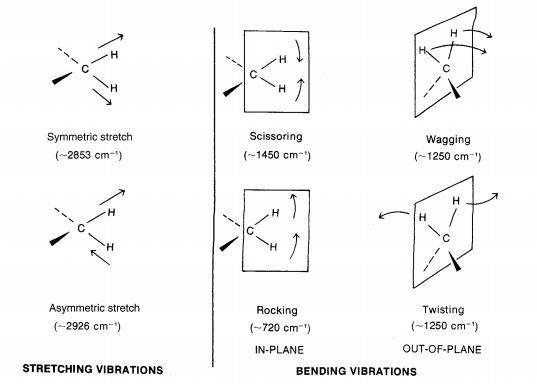
\includegraphics[scale=1]{Billeder/streak}
\end{center}
 
Det gælder desuden, at for et hvilket som helst molekyle, der er større eller har netop 3 atomer, hvor 2 af dem er ens at der er en asymmetrisk og en symmetrisk node. 
\\

Lad os nu se på hvordan vi kan beregne bølgetal for bestemte atom- og funktionelle grupper. Hvis vi nu ser på et af de simpleste eksempler for vibrationelle noder, et diatomisk molekyle med en strækkende vibration, kan vi betragte den kovalente binding mellem de to atomer som en fjeder. Et diatomisk molekyle kan betragtes som en fjeder hvor båndlængden bliver ved med at ændre sig. Dette betyder nødvendigvis at den kovalente binding, eller fjederen, må have en frekvens som den vibrerer med. Det gælder at energien for en harmonisk oscillator er direkte proportionelt med frekvensen for den harmoniske oscillator givet ved formlen (spectroscopy s. 18)

\begin{center}
\begin{equation}
E_{osc} \propto \upsilon_{osc}
\end{equation}
\end{center}

For et diatomisk molekyle er det, der bestemmer frekvensen i den harmonisk oscillerende bevægelse størrelserne, K (fjederkonstanten) og masserne af de to atomer der indgår i bindingen $m_1$ og $m_2$.
\\
Men da er frekvensen for en harmonisk oscillator er givet ved formlen

\begin{center}
\={v}$= \dfrac{1}{2 \pi c} \sqrt[2]{\dfrac{K}{\mu}}$
\end{center}

Denne formel er udledt fra Hookes lov for vibrerende fjedre. (FODNOTE TIL s8 spectroscopy). her er K, fjederkonstanten, \={v} er bølgetallet og $\mu$ er den reducerede masse givet ved formlen $\mu = \frac{m_1 m_2}{m_1 + m_2}$. Vi vil lige diskutere betydningen af K. 
\subsection{Fjederkonstanten for bindingen mellem diatomiske molekyler}

I normale fjedre vil fjederkonstanten, som navnet antyder, være konstant lige gyldigt hver vi hænger i den. Dette gør sig egentligt også gældende for de kovalente bindinger mellem molekyler, hvis de vel at mærke er underlagt præcist de samme betingelser. Så kovalente bånd er ikke én fjeder, men adskillige vis af forskellige fjedre og dette er utroligt vigtigt at have i mente, når vi skal se på forskellige værdier af K. Det gælder nemlig som en grov regel at værdien af fjederkonstanten, K, er tre gange så høj for tripeltbindinger som for enkeltbindinger og at K er dobbelt så høj for dobbeltbindinger som for enkeltbindinger. Vi sætter disse værdier af K til at være henholdsvis 5, 10 og 15 for enkelt-, dobbelt- og trippeltbindinger. Vi vil senere diskutere i hvor stor grad denne grove fingerregel for beregninger af bølgetal holder.
\\

Vi skal imidlertid straks notere os et par ting. For det første vil et større K medfører et større bølgetal, da tælleren bliver større og værdien for $\sqrt[2]{\dfrac{K}{\mu}}$ da bliver større. For det andet vil store atomer der er bundet til atomer der er relativt mindre til dem selv vibrerer ved højere frekvenser da værdien af $\mu$ vil være mindre og gøre $\sqrt[2]{\dfrac{K}{\mu}}$ større. 
\\

Vi kan tjekke om dette passer ved at slå op i en databog og se på bølgetal for forskellige atomer bundet sammen:
\\
\includegraphics[scale=1]{Billeder/udklip}

Vi kan se jo større et atom som carbon er bundet til jo større bliver $\mu$ og derfor også bølgetallet \={v}.

Bevægelser mellem atomer, der bøjende vil også optræde ved en lavere energi, og altså også ved et lavere \={v}, end de strækkende bevægelser. Eksempelvis vil C-H stræk give udslag ved et bølgetal på ca. 3000 $cm^{-1}$ mens C-H bøj vil give et udsalg omkring $1340cm^{-1}$. 




